\documentclass{beamer}
\usetheme{metropolis}
\usepackage{graphicx}
\usepackage{subfig}
\usepackage{tcolorbox}
\title{Finite State Machines and COVID-19}
\author{Jordan Hanson}
\institute{Whittier College Department of Physics and Astronomy}

\begin{document}
\maketitle

\section{Summary}

\begin{frame}{Finite State Machines and COVID-19}
\begin{enumerate}
\item Finite State Machines (FSMs)
\begin{itemize}
\item Inputs, outputs, and states
\item State diagram
\item Transitions
\end{itemize}
\item \textbf{COVID-19 as an FSM}
\begin{itemize}
\item Python3 exercise, apply concepts to real world
\item Object-oriented design
\item Game theory, rules of the game
\end{itemize}
\item Results
\begin{itemize}
\item Exponential growth
\item Social distancing
\item \alert{Second waves}
\end{itemize}
\end{enumerate}
\end{frame}

\section{Finite State Machines}

\begin{frame}{Finite State Machines}
\textit{Finite State Machine}: is a mathematical model of computation. It is an abstract machine that can be in exactly one of a finite number of states at any given time.
\begin{enumerate}
\item FSM can change from one state to another in response to inputs (transitions)
\item Requires initial state and mapping of inputs to transitions
\end{enumerate}

\begin{itemize}
\item Inputs - a small list of binary bits
\item Outputs - a small list of binary bits
\item States - $2^n - 1$ states represented by $n$ bits
\end{itemize}
\end{frame}

\begin{frame}{Finite State Machines}
\textbf{The State Diagram}: table or chart defining input-transition map.
\begin{table}
\centering
\begin{tabular}{| c | c | c | c |}
\hline
input & state & next state & output \\ \hline \hline
0 & 00 & 11 & 1 \\ \hline
1 & 00 & 01 & 1 \\ \hline
0 & 01 & 00 & 1 \\ \hline
1 & 01 & 10 & 1 \\ \hline
0 & 10 & 00 & 1 \\ \hline
1 & 10 & 01 & 1 \\ \hline
0 & 11 & 11 & 0 \\ \hline
1 & 11 & 01 & 1 \\ \hline
\end{tabular}
\end{table}
\end{frame}

\begin{frame}{Finite State Machines}
\textbf{The State Diagram}: table or chart defining input-transition map.
\begin{figure}
\centering
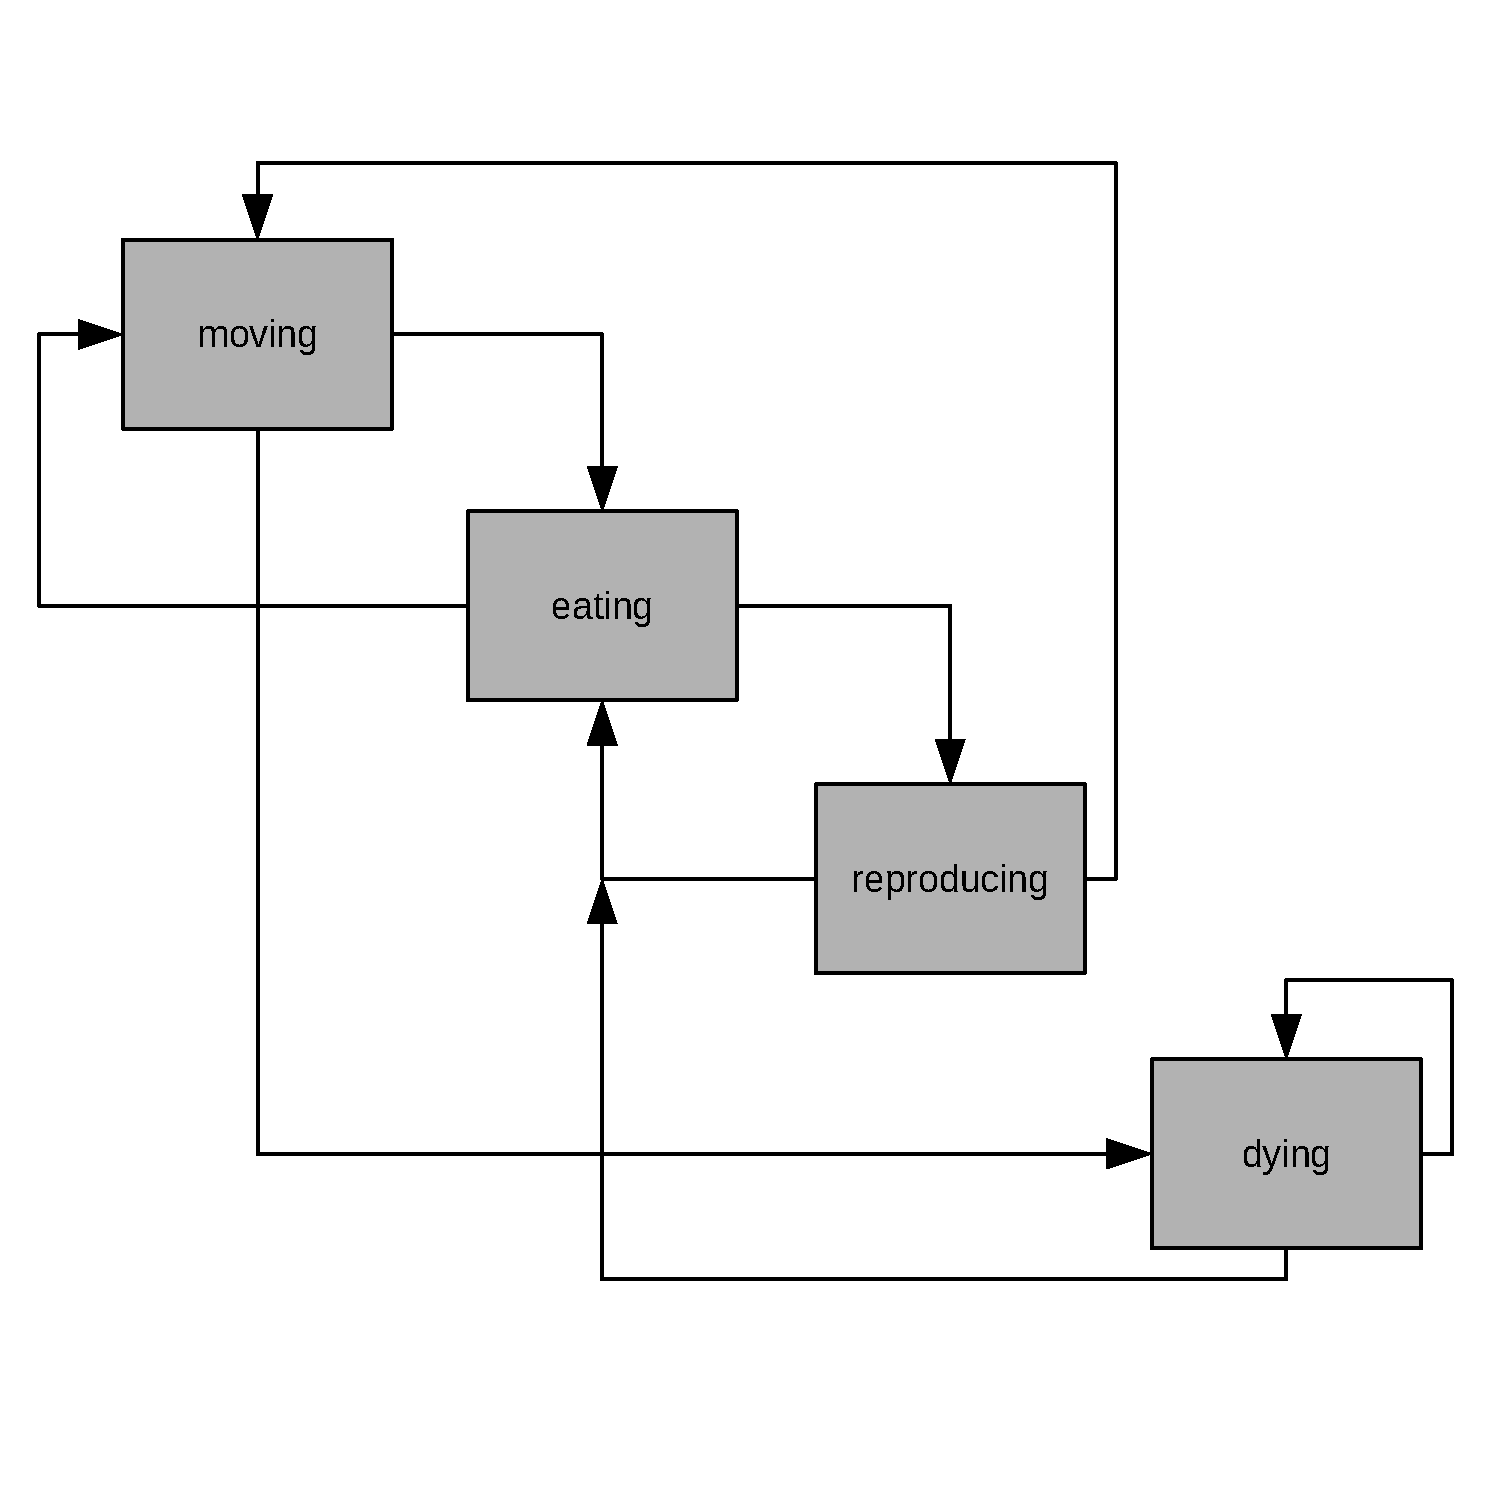
\includegraphics[width=0.5\textwidth]{figures/state_diagram.pdf}
\caption{\label{fig:state1} A state-diagram for our virus model.}
\end{figure}
\end{frame}

\section{COVID-19 as an FSM}

\begin{frame}{COVID-19 as an FSM}
\begin{figure}
\centering
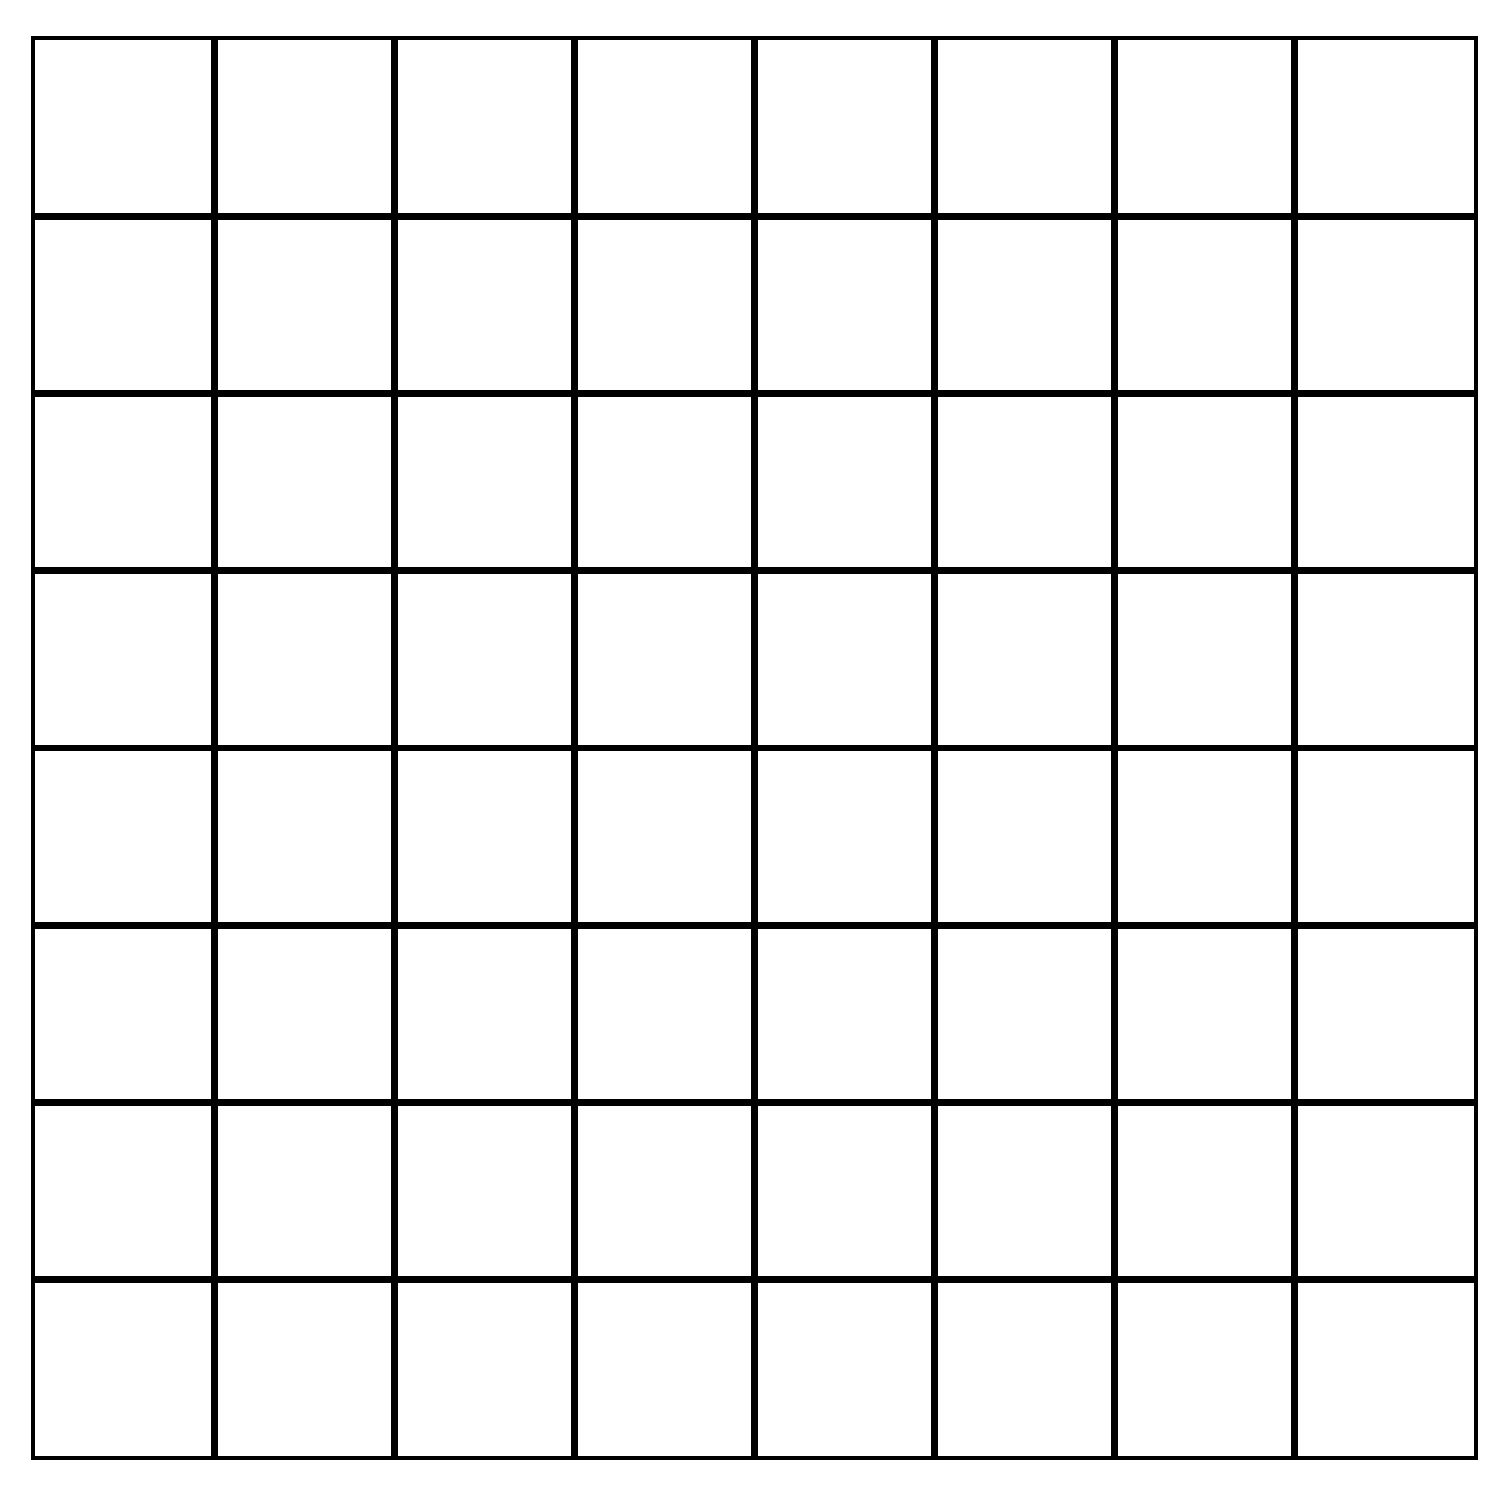
\includegraphics[width=0.5\textwidth]{figures/grid.pdf}
\caption{\label{fig:grid1} The basic grid where the FSMs live.}
\end{figure}
\end{frame}

\begin{frame}{COVID-19 as an FSM}
\begin{figure}
\centering
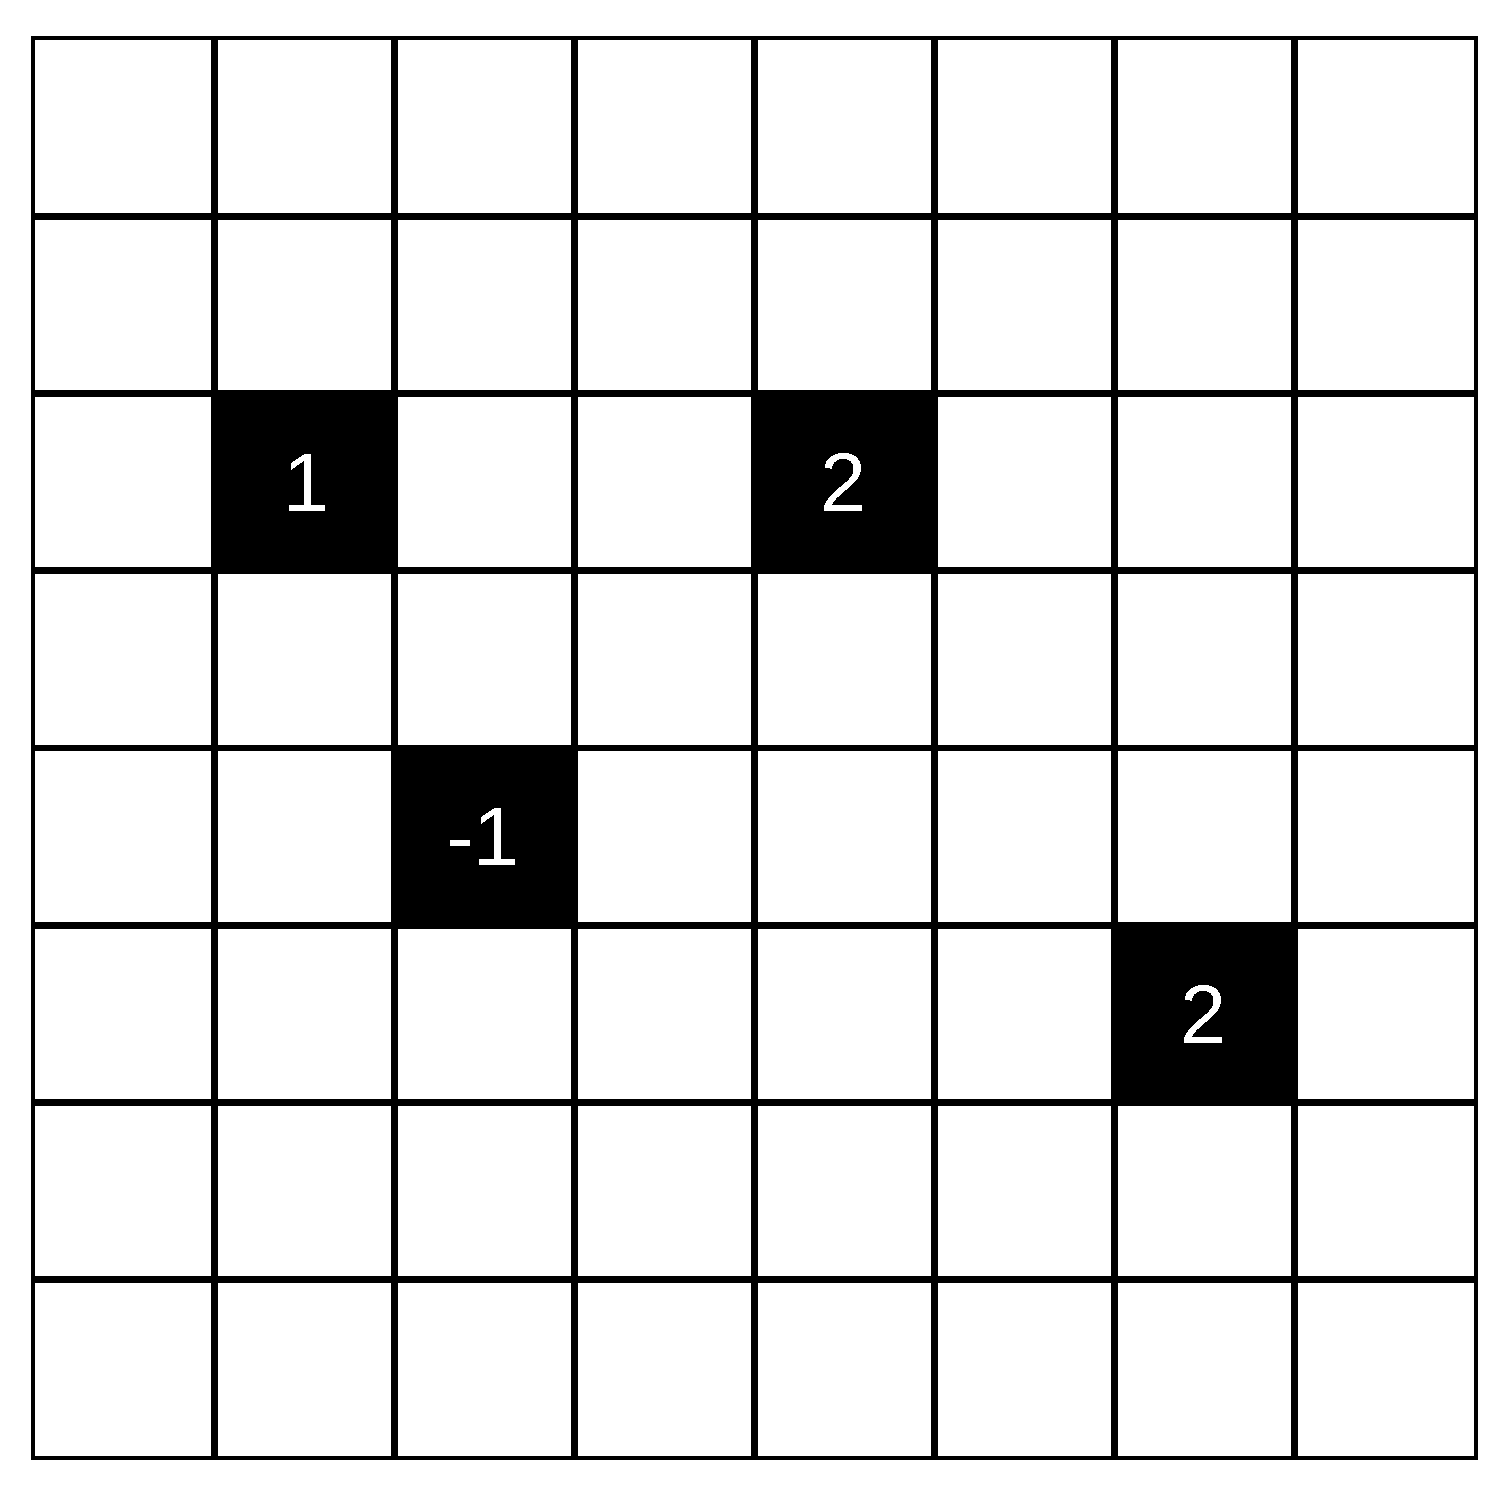
\includegraphics[width=0.5\textwidth]{figures/grid_food.pdf}
\caption{\label{fig:grid2} The basic grid where the FSMs live.}
\end{figure}
\end{frame}

\begin{frame}{COVID-19 as an FSM}
\begin{figure}
\centering
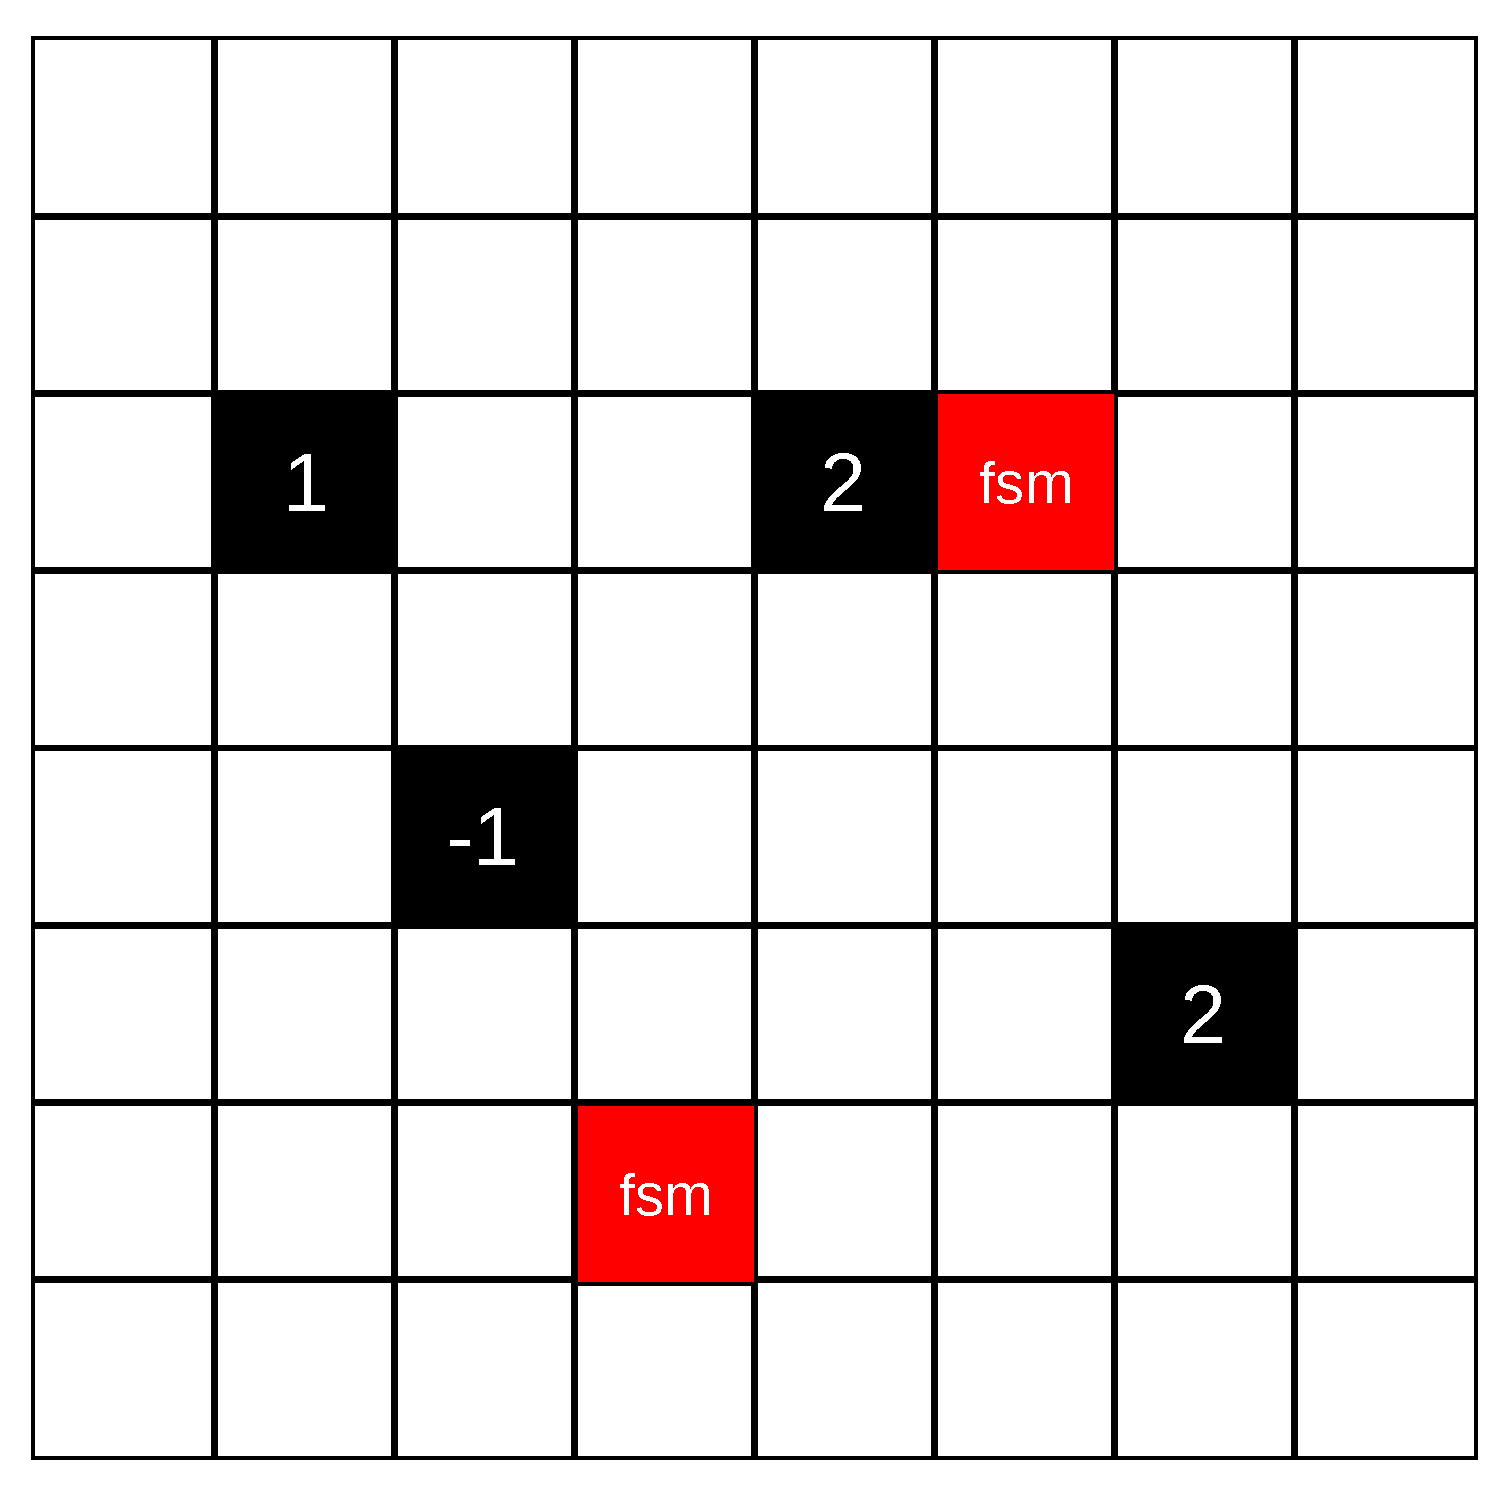
\includegraphics[width=0.5\textwidth]{figures/grid_food_fsm.pdf}
\caption{\label{fig:grid3} The basic grid where the FSMs live.}
\end{figure}
\end{frame}

\begin{frame}{COVID-19 as an FSM}
\begin{figure}
\centering
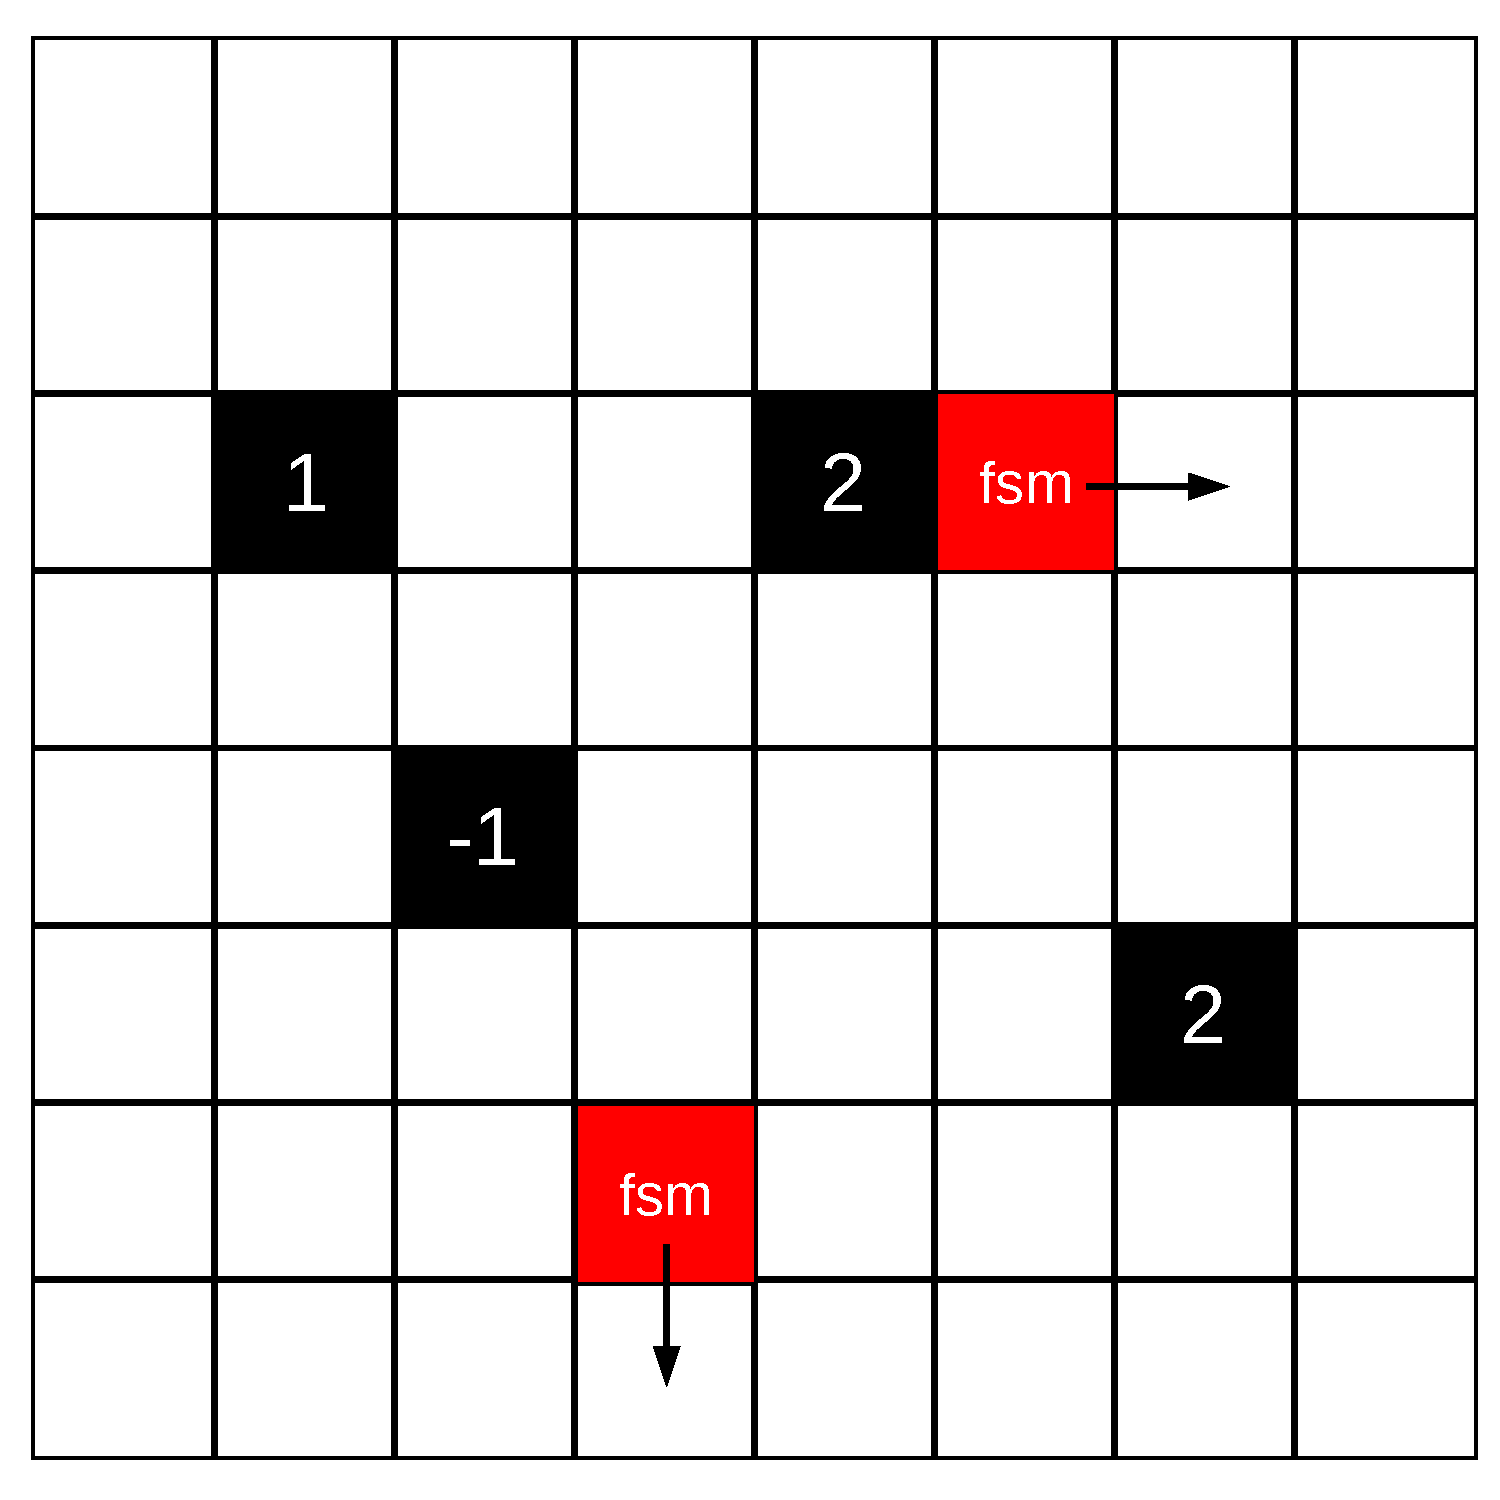
\includegraphics[width=0.5\textwidth]{figures/grid_food_fsm_move.pdf}
\caption{\label{fig:grid4} The basic grid where the FSMs live.}
\end{figure}
\end{frame}

\begin{frame}{COVID-19 as an FSM}
\begin{figure}
\centering
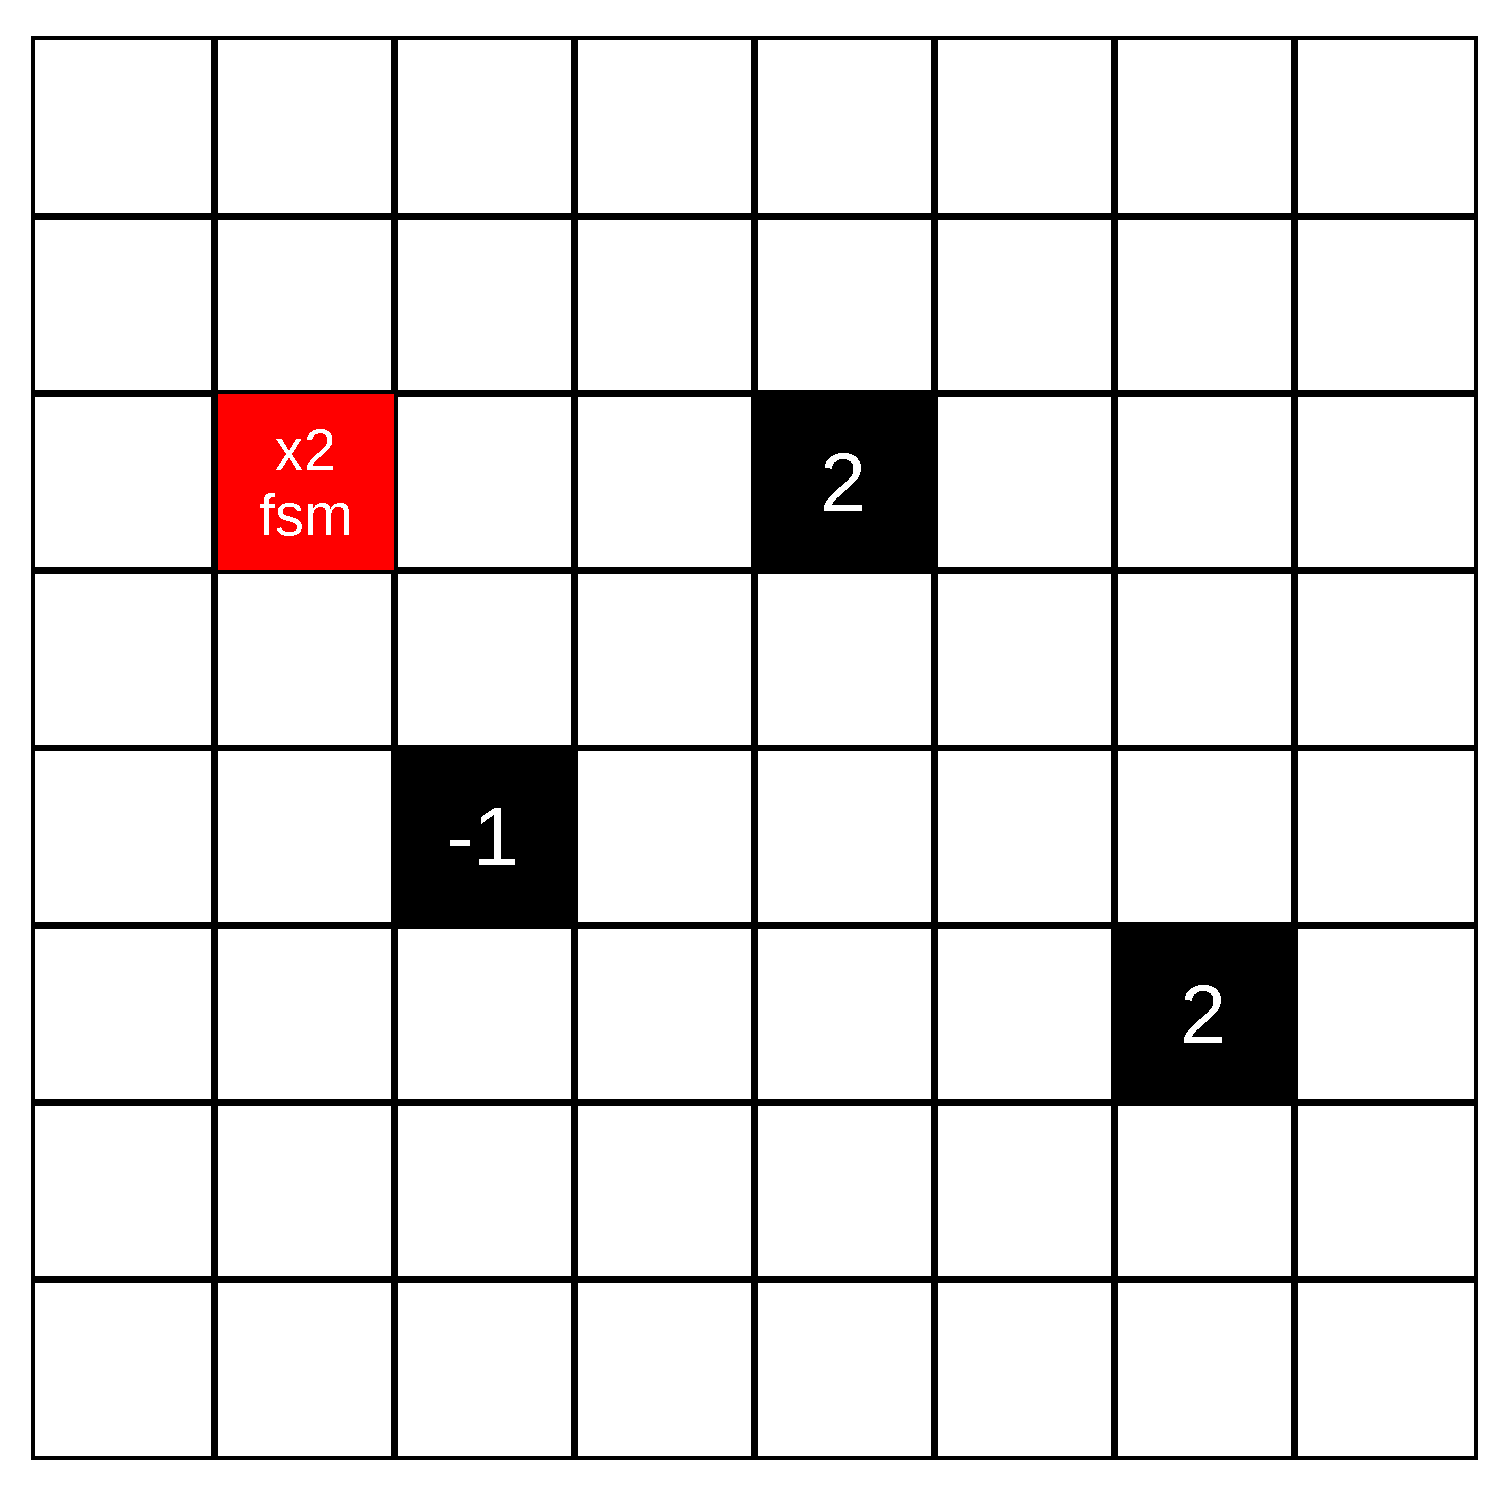
\includegraphics[width=0.5\textwidth]{figures/grid_food_fsm_reproduce.pdf}
\caption{\label{fig:grid5} The basic grid where the FSMs live.}
\end{figure}
\end{frame}

\begin{frame}{COVID-19 as an FSM}
\begin{figure}
\centering
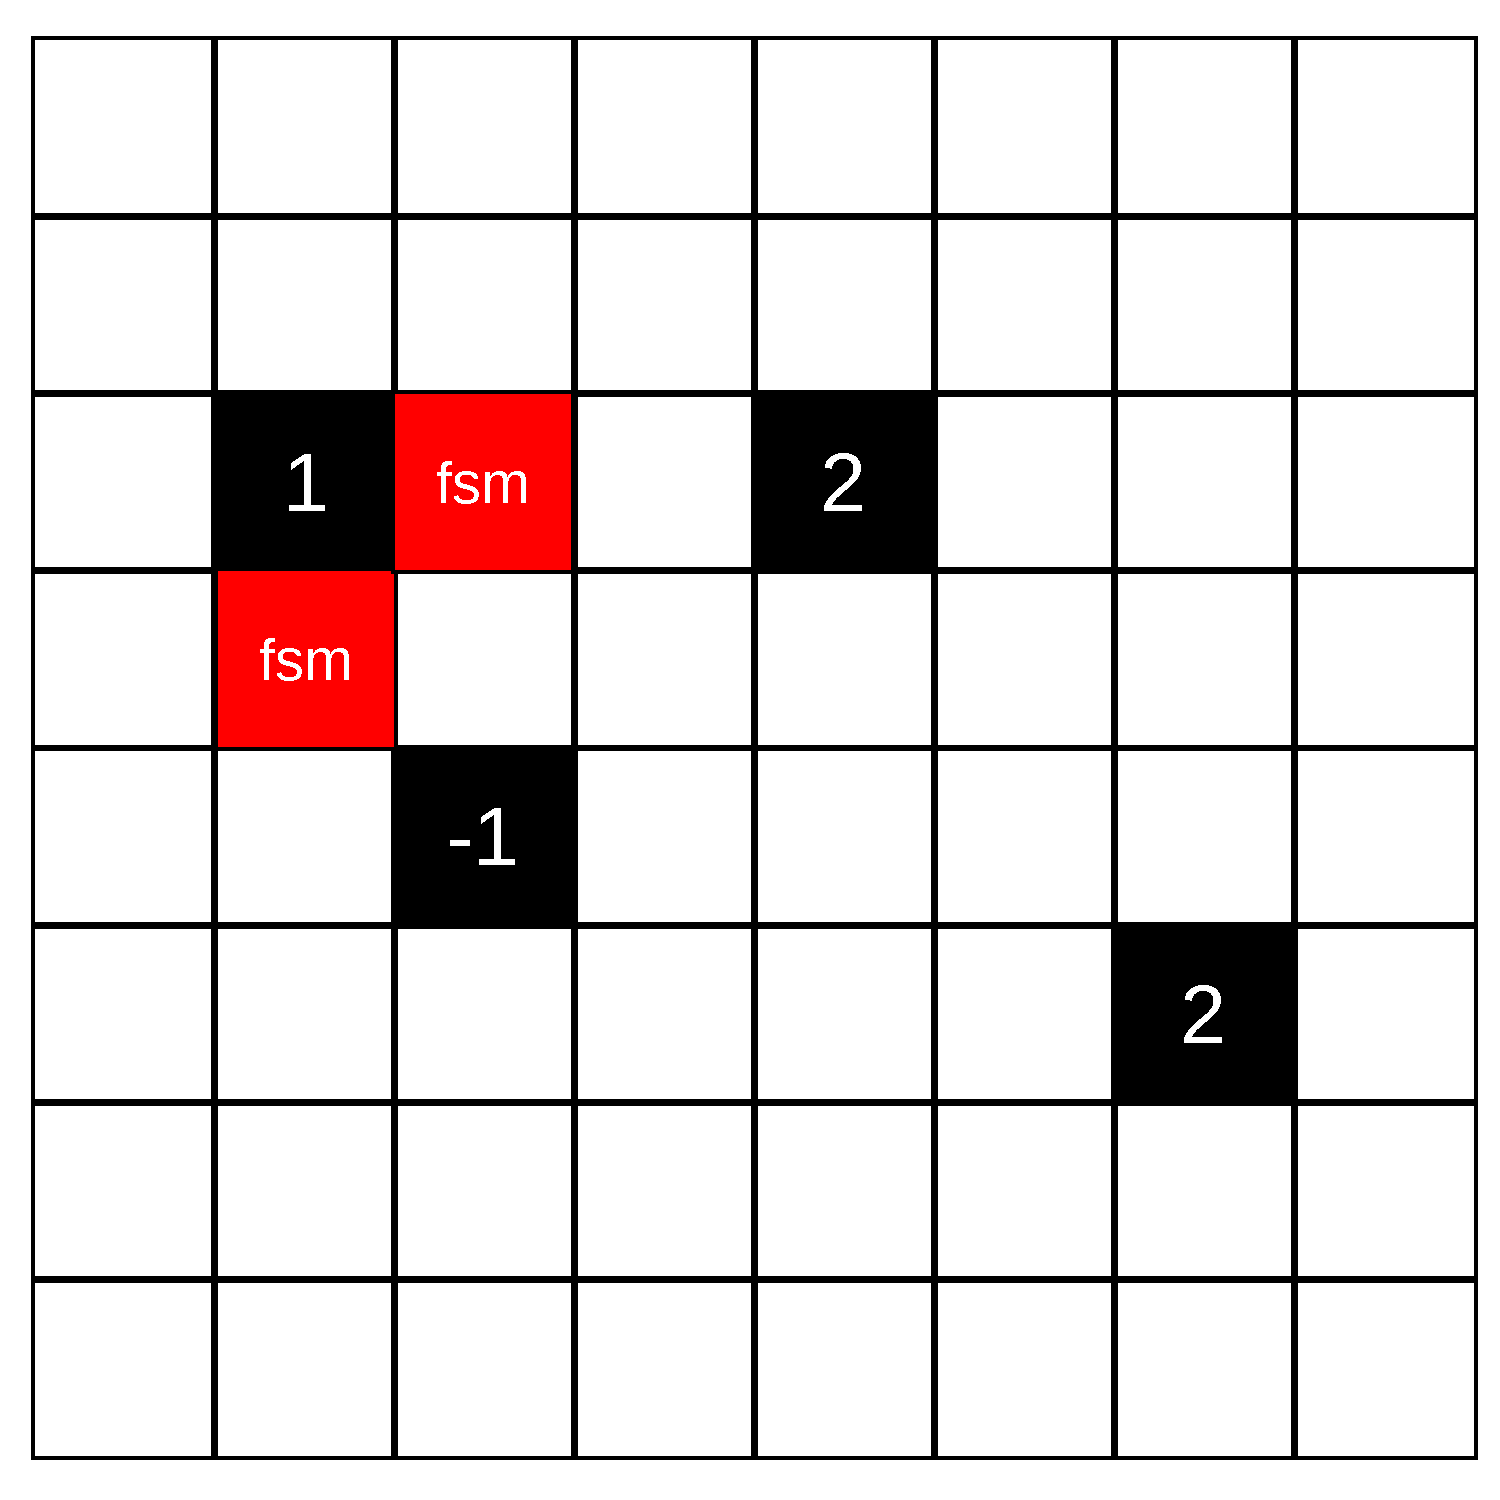
\includegraphics[width=0.5\textwidth]{figures/grid_food_fsm_moveRepr.pdf}
\caption{\label{fig:grid6} The basic grid where the FSMs live.}
\end{figure}
\end{frame}

\section{Results}

\begin{frame}{Results}
\begin{figure}
\centering
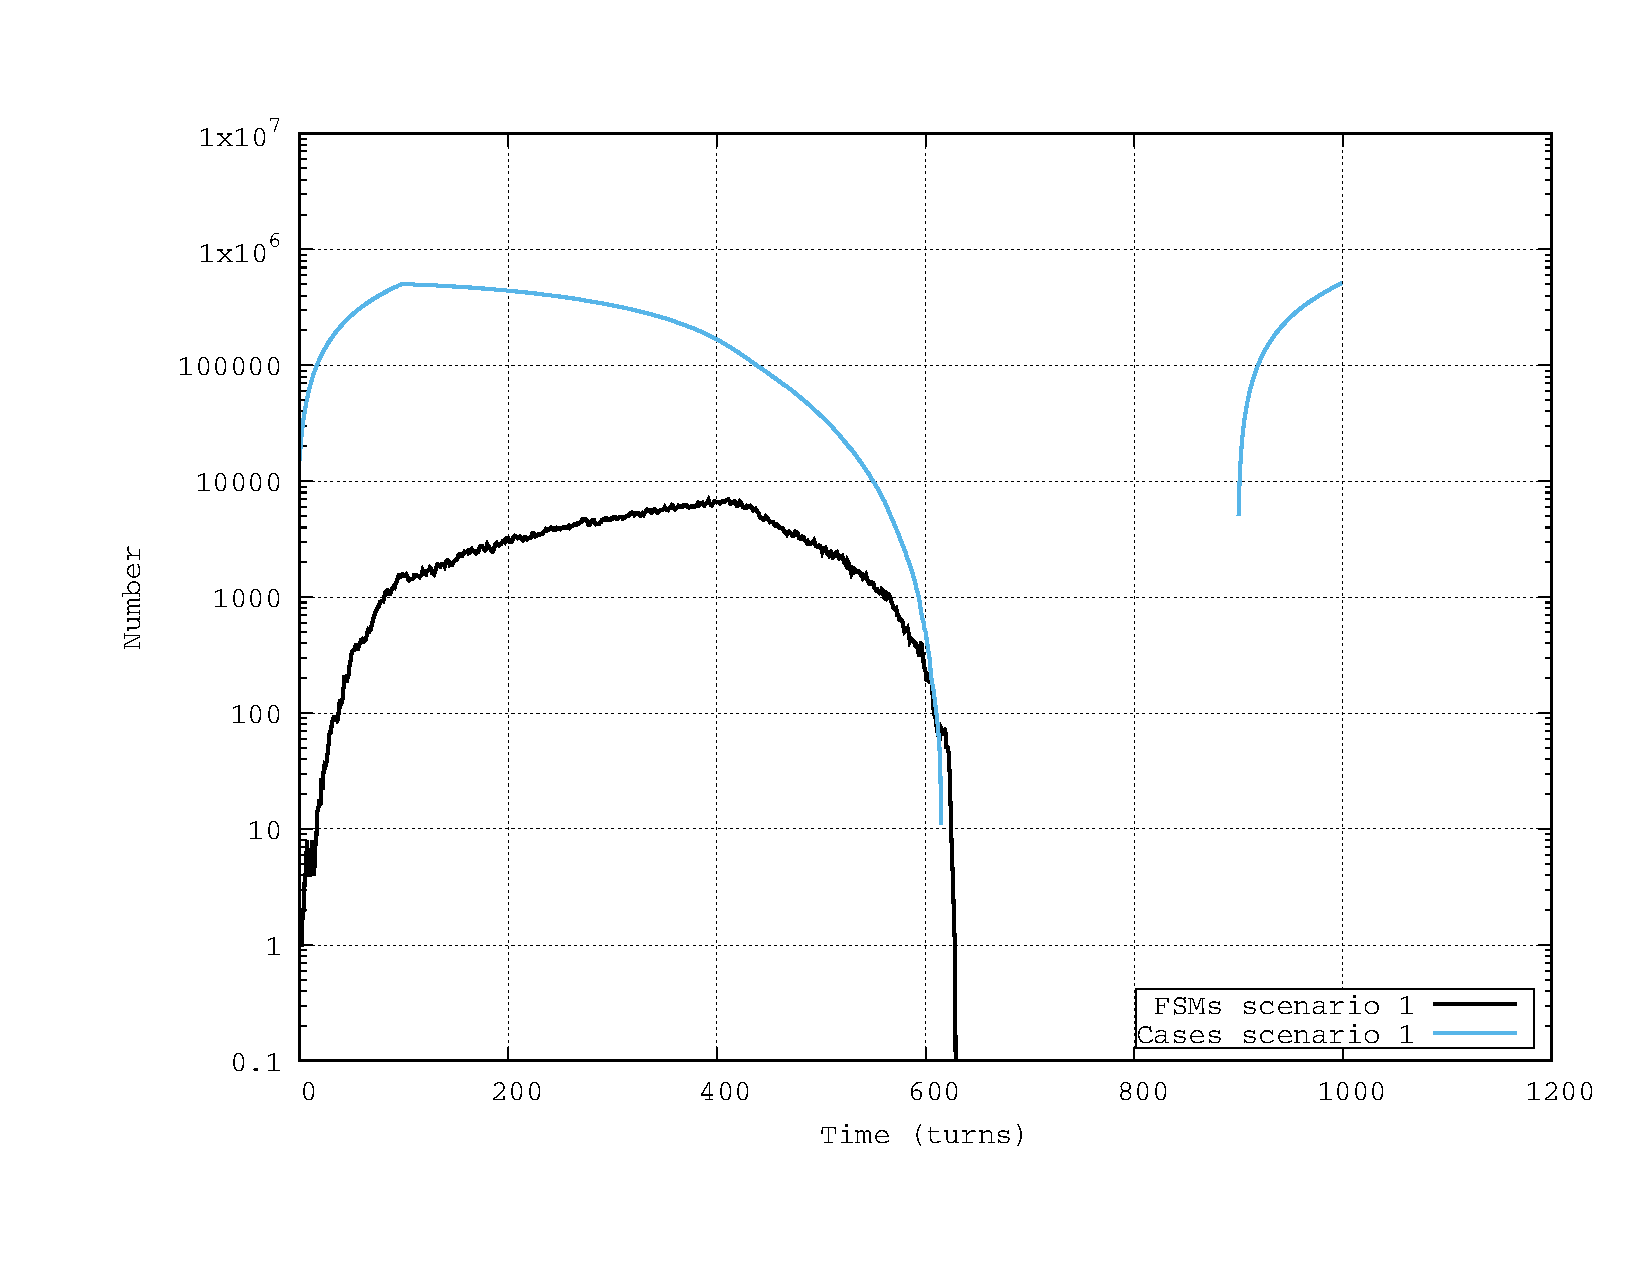
\includegraphics[width=0.85\textwidth]{figures/April23_plot1.pdf}
\caption{\label{fig:fsm} Scenario 1.}
\end{figure}
\end{frame}

\begin{frame}{Results}
\begin{figure}
\centering
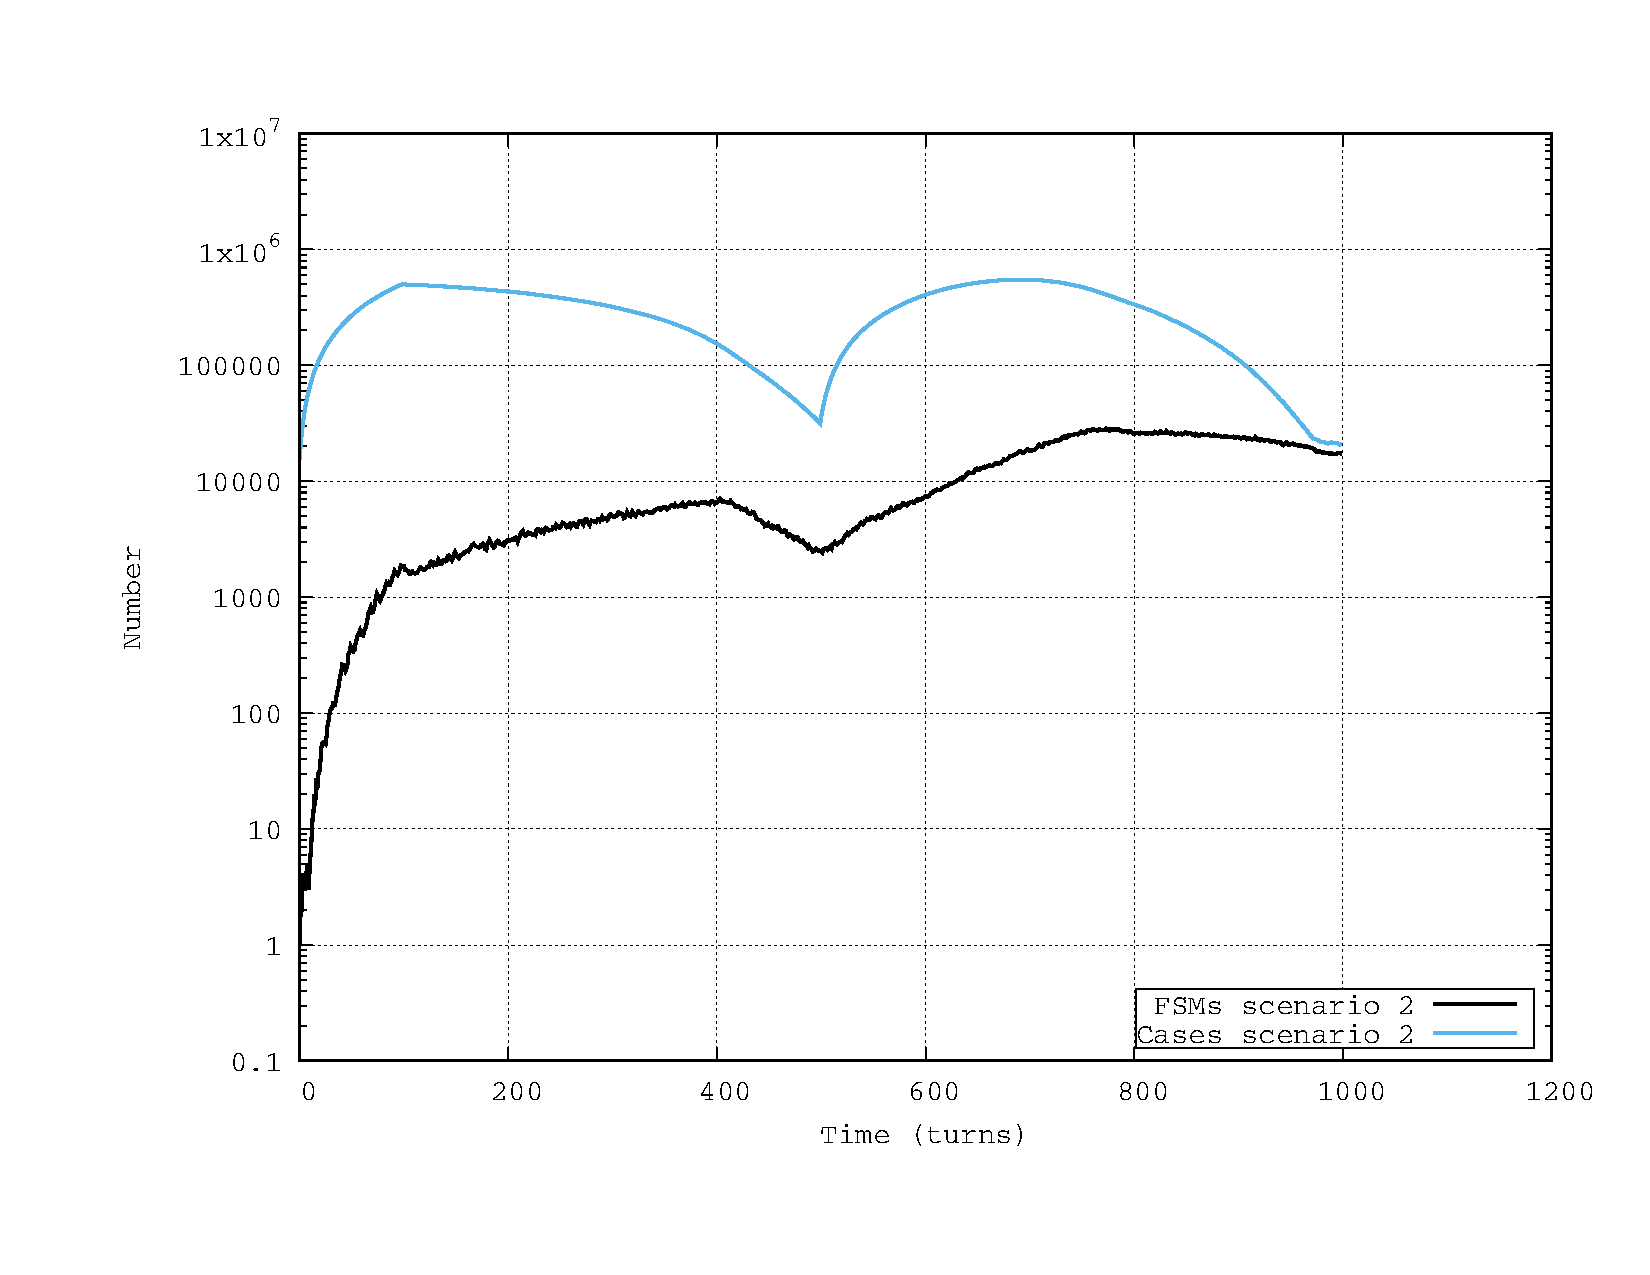
\includegraphics[width=0.85\textwidth]{figures/April23_plot2.pdf}
\caption{\label{fig:fsm2} Scenario 2.}
\end{figure}
\end{frame}

\section{Conclusion}

\begin{frame}{Finite State Machines and COVID-19}
\begin{enumerate}
\item Finite State Machines (FSMs)
\begin{itemize}
\item Inputs, outputs, and states
\item State diagram
\item Transitions
\end{itemize}
\item \textbf{COVID-19 as an FSM}
\begin{itemize}
\item Python3 exercise, apply concepts to real world
\item Object-oriented design
\item Game theory, rules of the game
\end{itemize}
\item Results
\begin{itemize}
\item Exponential growth
\item Social distancing
\item \alert{Second waves}
\end{itemize}
\end{enumerate}
\end{frame}

\end{document}
